\begin{appendix}

    \chapter{Abbildungen}

        \begin{figure}[ht]
            \centering
            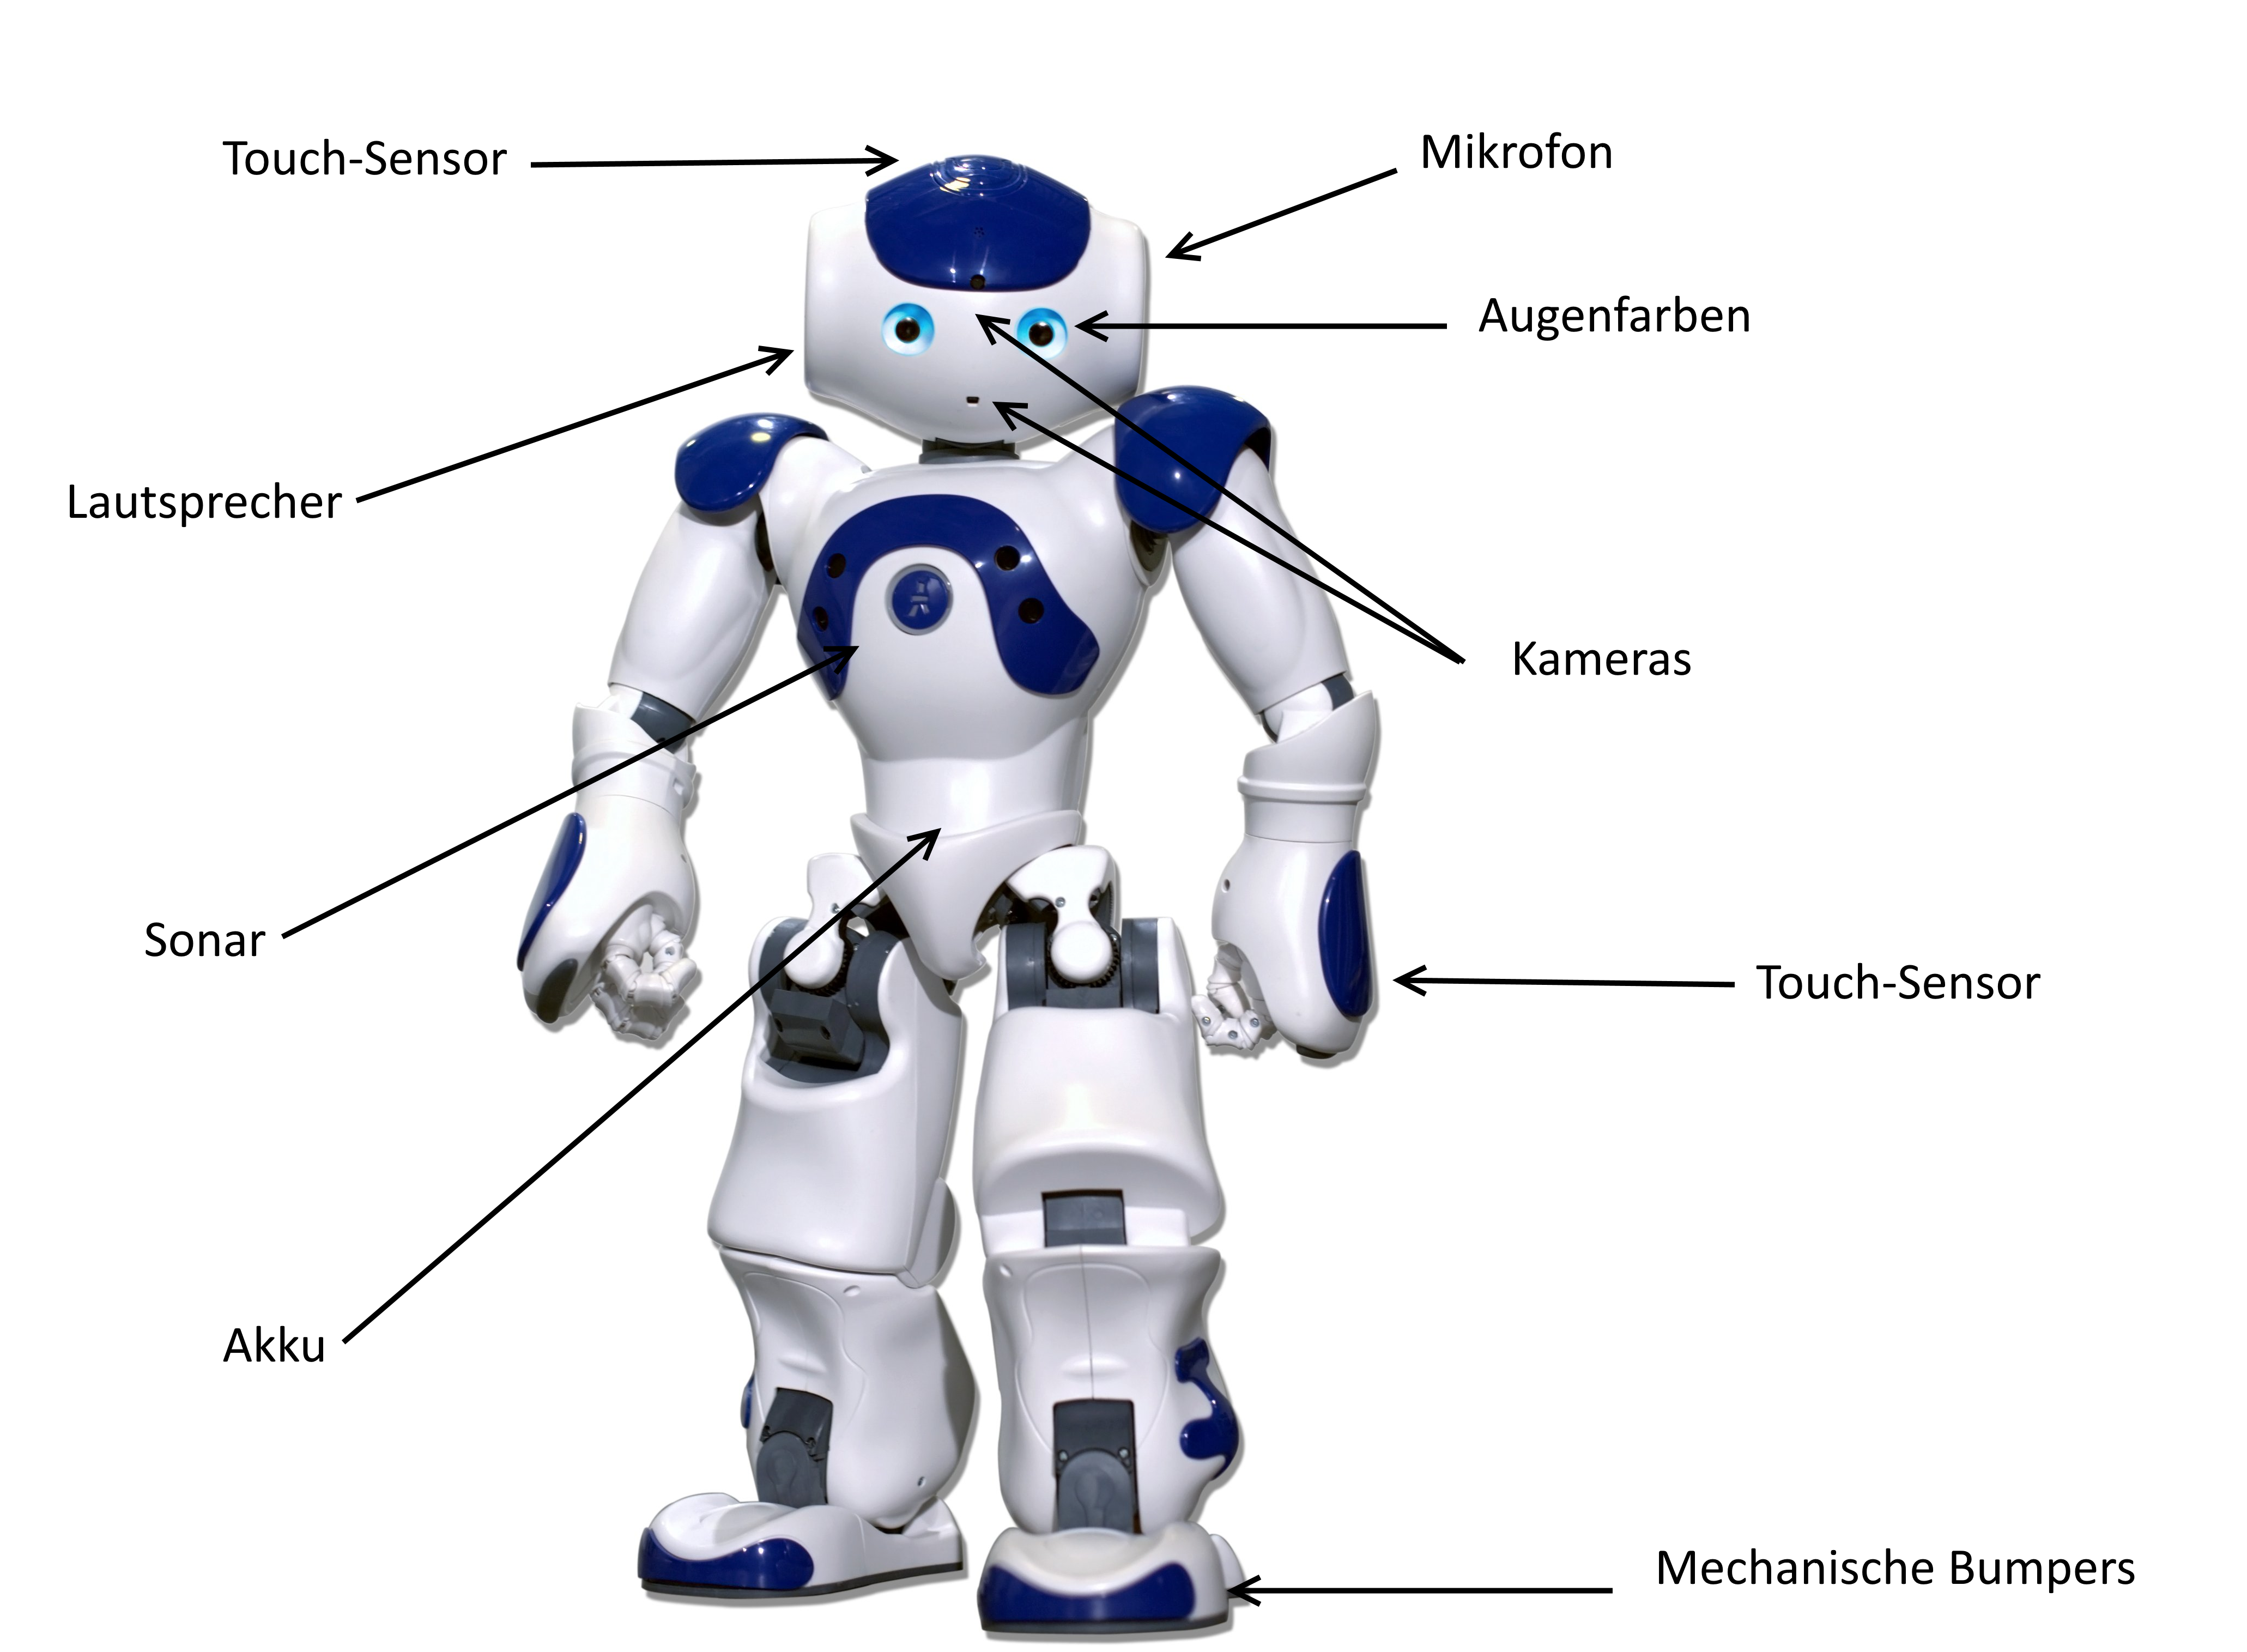
\includegraphics[width=0.99\textwidth]{src/pictures/nao-sensors.png}
            \caption{Sensoren des NAO}
            \label{img:nao:sensors}
        \end{figure}

        \begin{figure}[ht]
            \centering
            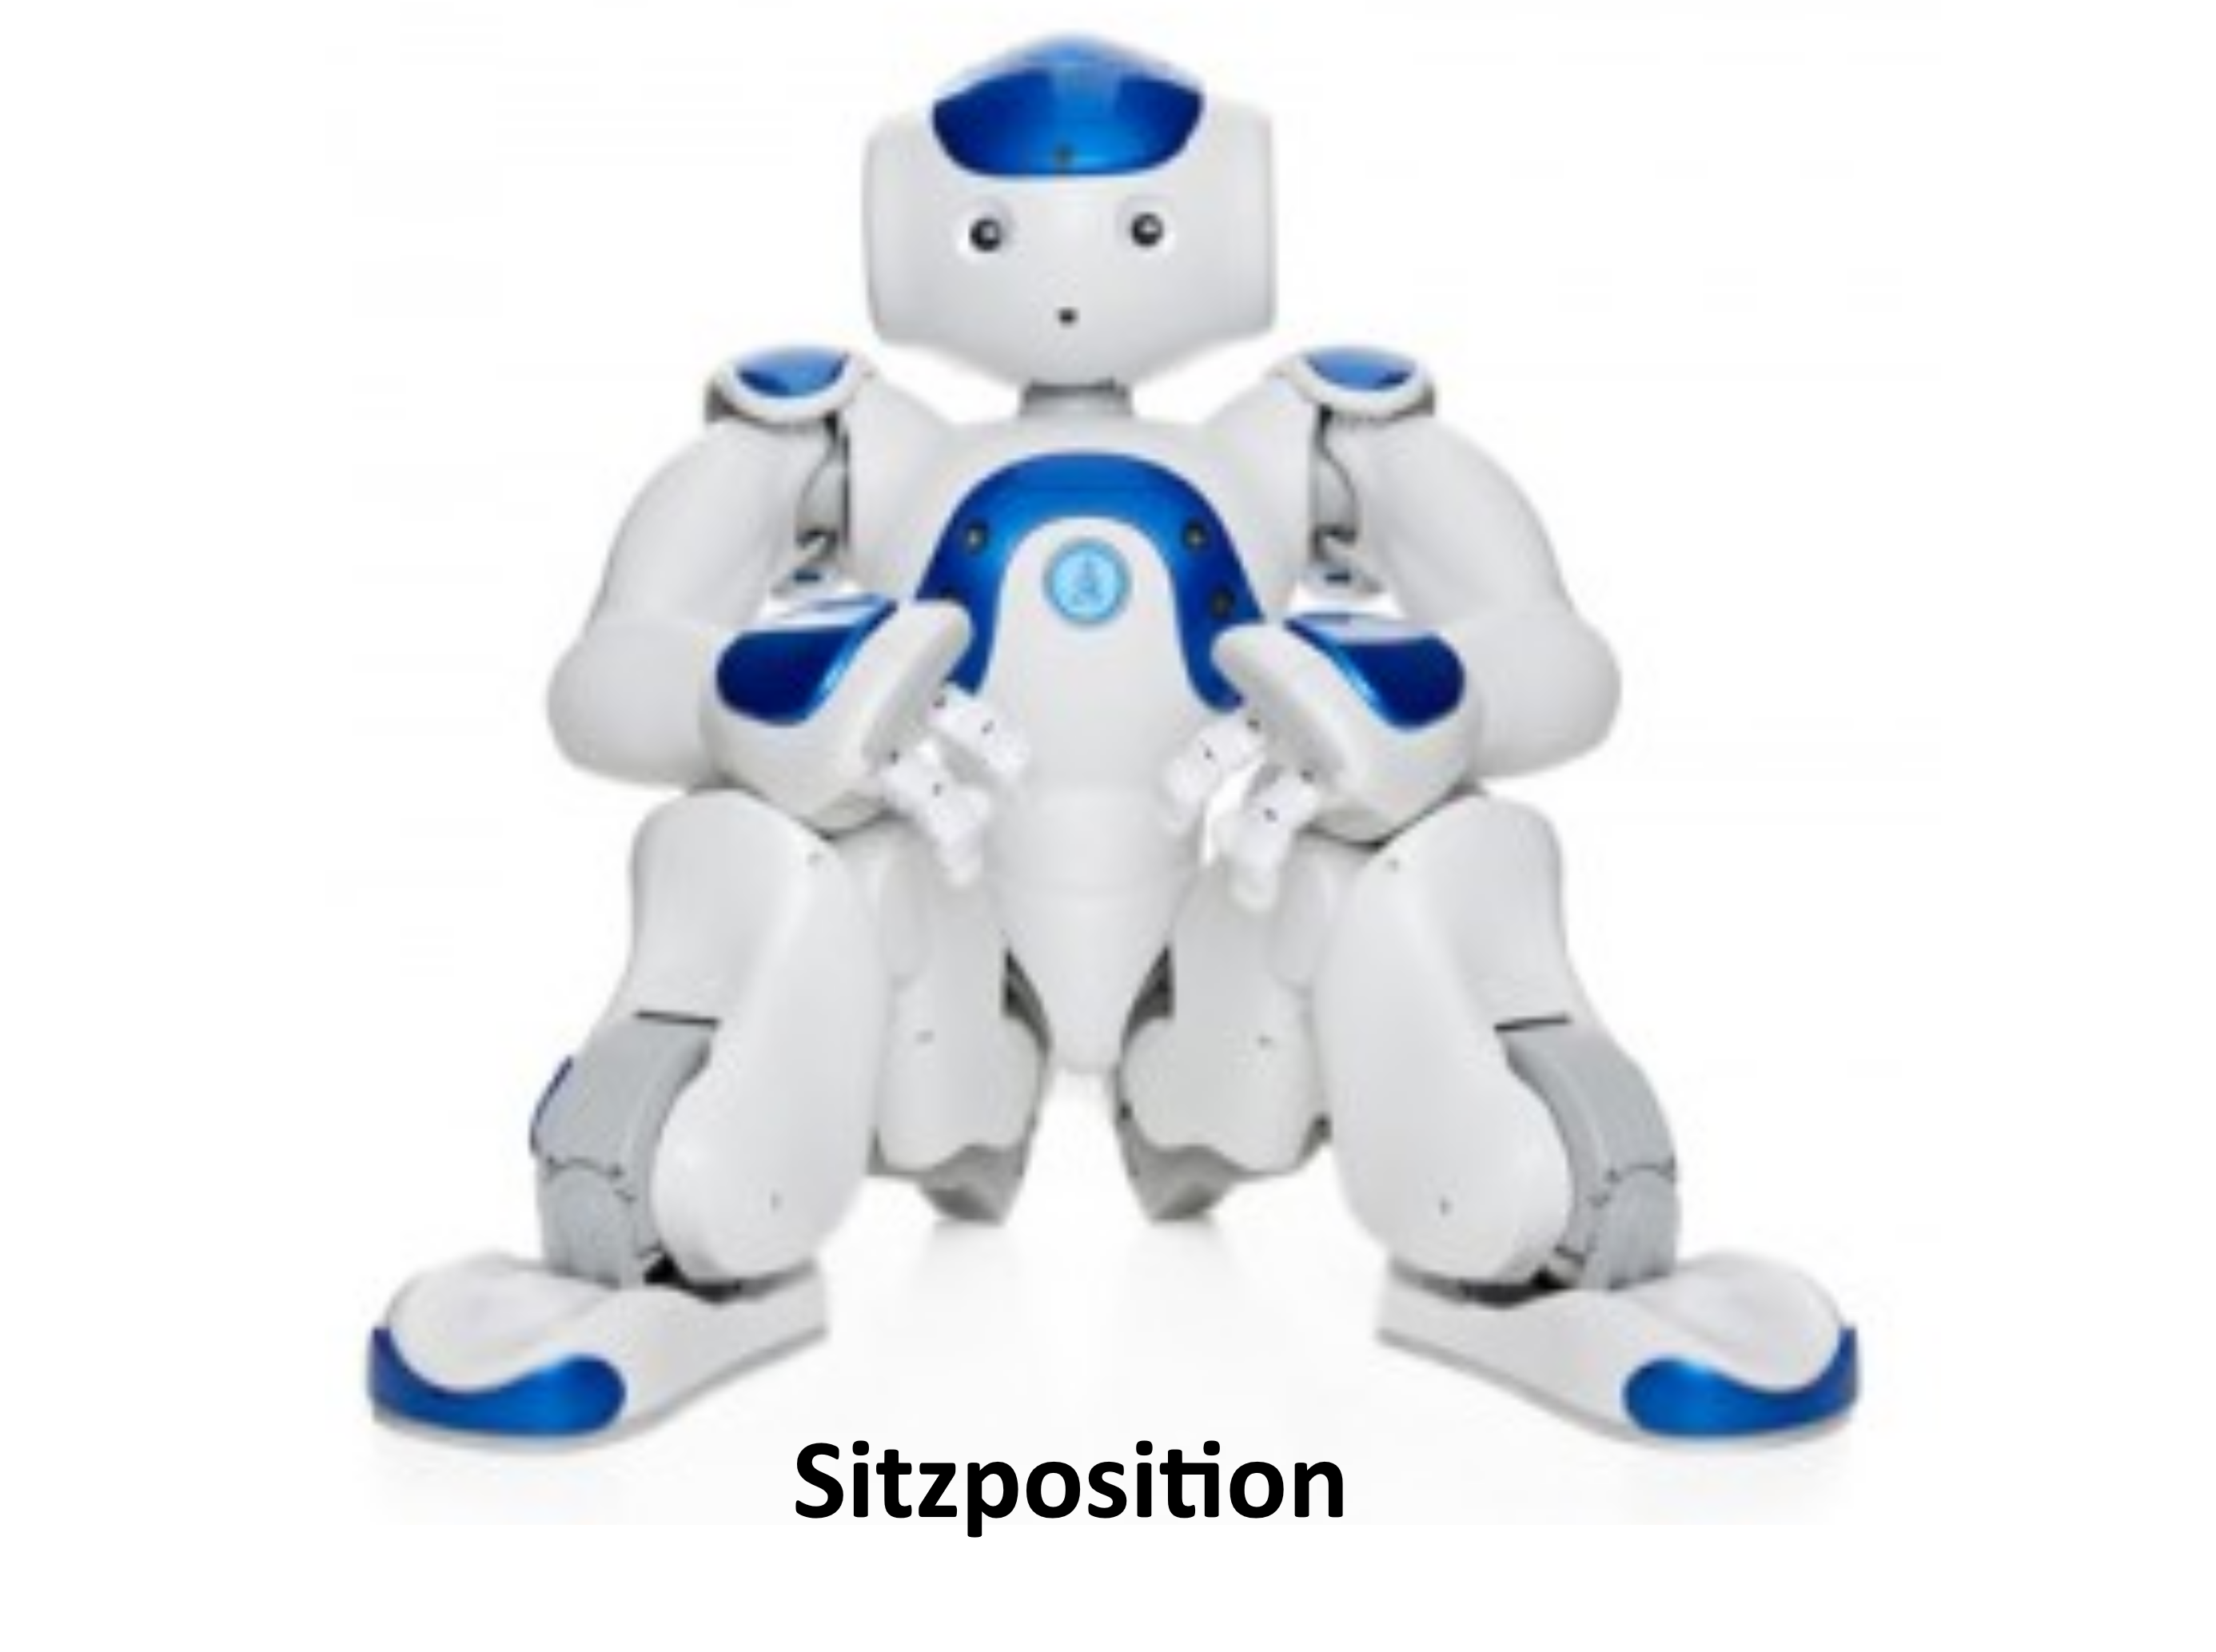
\includegraphics[width=0.99\textwidth]{src/pictures/nao-sitting.png}
            \caption{Sitzposition des NAO}
            \label{img:nao:sitting}
        \end{figure}

        \begin{figure}[ht]
            \centering
            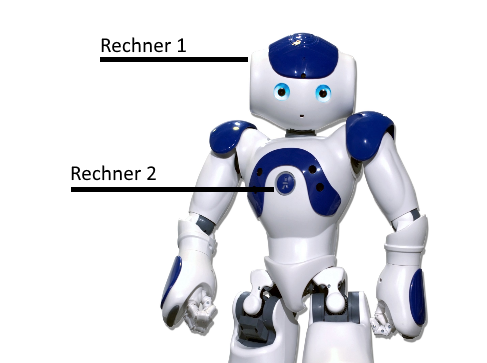
\includegraphics[width=0.99\textwidth]{src/pictures/nao-computers.png}
            \caption{Recheneinheiten des NAO}
            \label{img:nao:computers}
        \end{figure}

        \begin{figure}[ht]
            \centering
            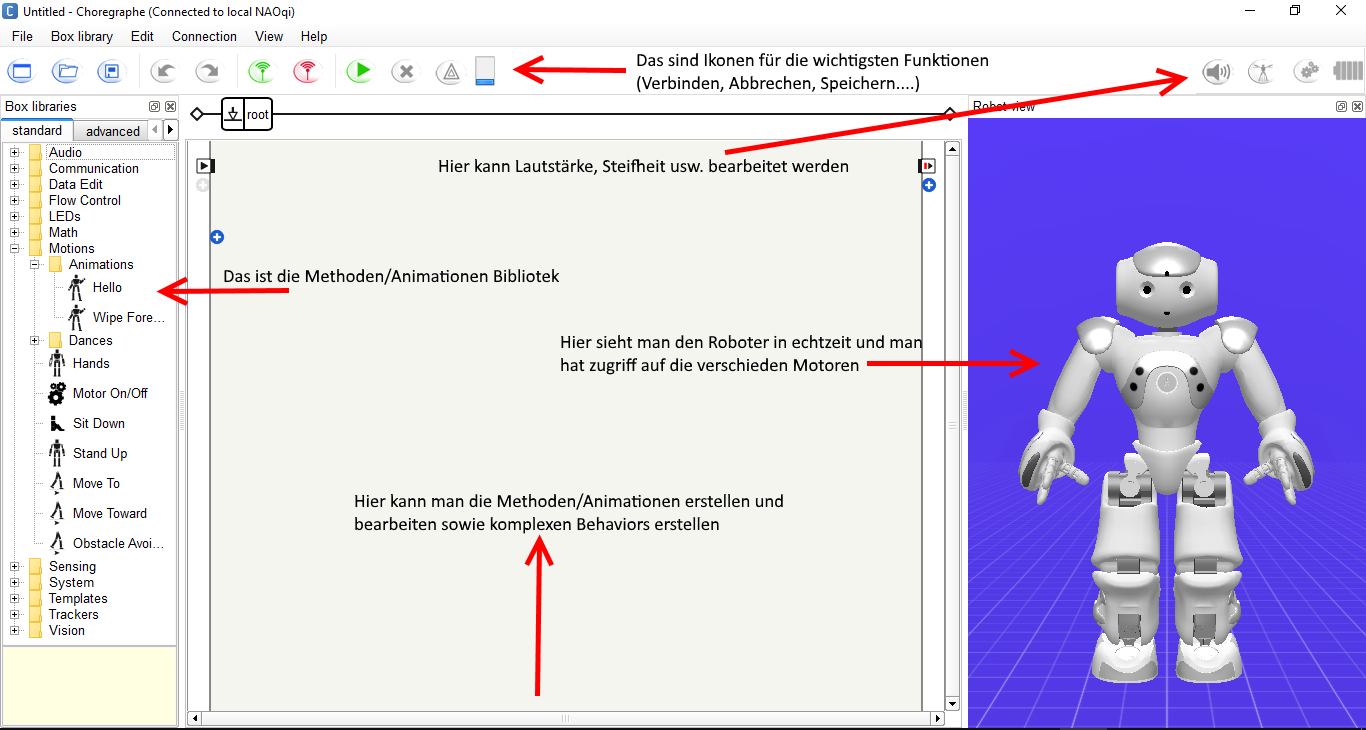
\includegraphics[angle=90, width=0.80\textwidth]{src/pictures/nao-choreo-welcome.png}
            \caption{Choreographe}
            \label{img:nao:choreo:welcome}
        \end{figure}

        \begin{figure}[ht]
            \centering
            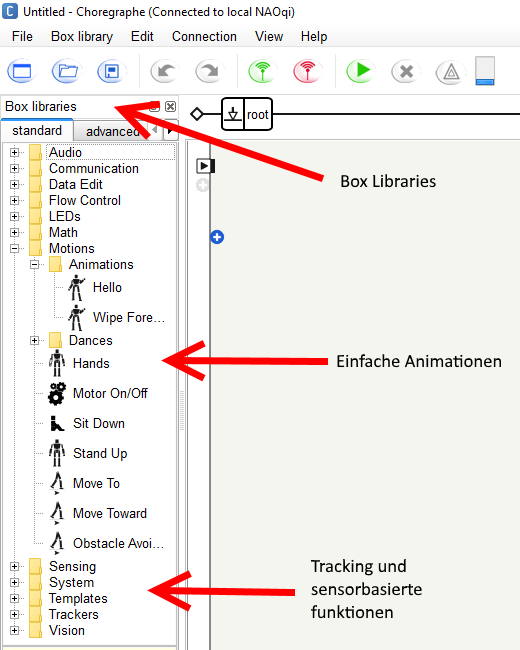
\includegraphics[width=0.99\textwidth]{src/pictures/nao-choreo-boxlib.png}
            \caption{Choreographe: Box Libraries}
            \label{img:nao:choreo:boxlib}
        \end{figure}

        \begin{figure}[ht]
            \centering
            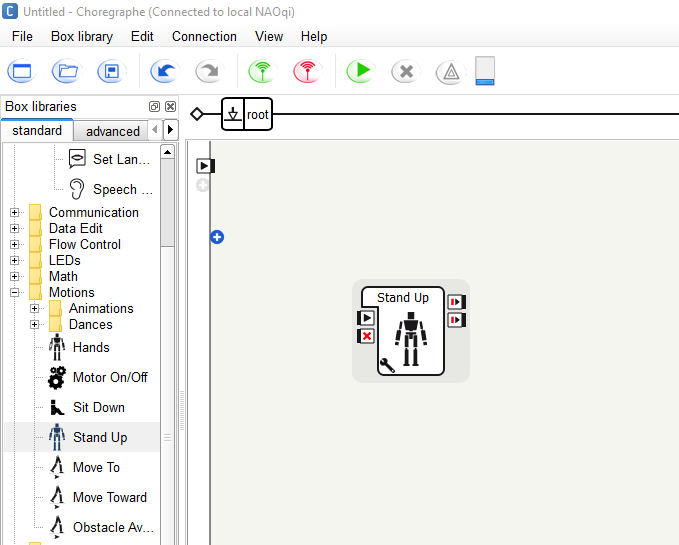
\includegraphics[width=0.99\textwidth]{src/pictures/nao-choreo-dad.png}
            \caption{Choreographe: Behaviour auf Arbeitsfläche}
            \label{img:nao:choreo:draganddrop}
        \end{figure}

        \begin{figure}[ht]
            \centering
            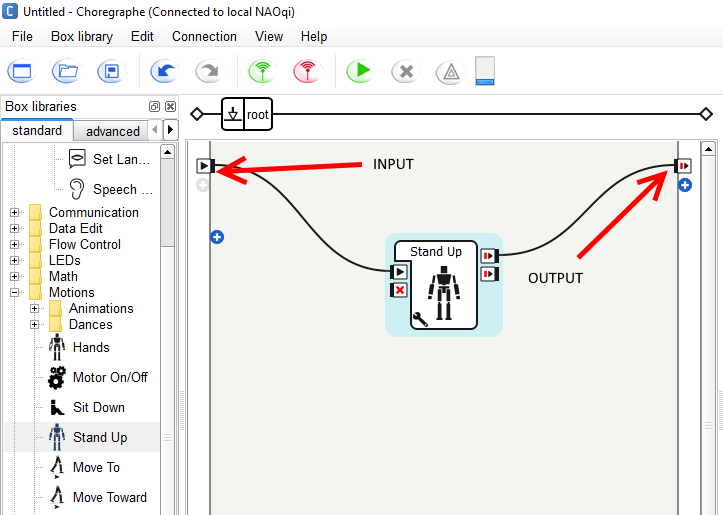
\includegraphics[width=0.99\textwidth]{src/pictures/nao-choreo-connect.png}
            \caption{Choreographe: Behaviour verbinden}
            \label{img:nao:choreo:connect}
        \end{figure}

        \begin{figure}[ht]
            \centering
            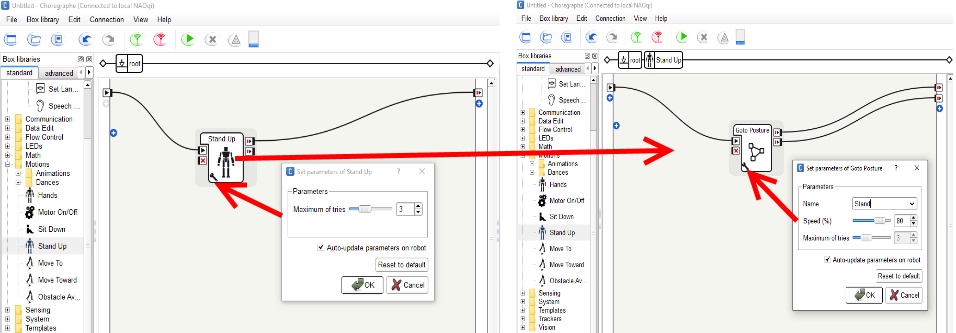
\includegraphics[width=0.99\textwidth]{src/pictures/nao-choreo-options.png}
            \caption{Choreographe: Behaviour bearbeiten}
            \label{img:nao:choreo:options}
        \end{figure}

        \cleardoubleemptypage

        \begin{figure}[ht]
            \centering
            \includegraphics[width=0.99\textwidth]{src/pictures/Packages-uml.png}
            \caption{Packages}
            \label{img:packages}
        \end{figure}

        \begin{figure}[ht]
            \centering
            \includegraphics[width=0.99\textwidth]{src/pictures/Package_Behaviour-uml.png}
            \caption{Package: Behaviour}
            \label{img:package:behaviour}
        \end{figure}

        \begin{figure}[ht]
            \centering
            \includegraphics[width=0.99\textwidth]{src/pictures/Package_OpenCV-uml.png}
            \caption{Package: OpenCV}
            \label{img:package:ocv}
        \end{figure}

        \cleardoubleemptypage

        \begin{figure}[ht]
            \centering
            \includegraphics[width=0.99\textwidth]{src/pictures/algo/usecase.png}
            \caption{Algorithmus: Usecases}
            \label{img:algo:usecases}
        \end{figure}

        \cleardoubleemptypage

        \begin{figure}[ht]
            \centering
            \includegraphics[width=0.99\textwidth]{src/pictures/Package_Algo-uml.png}
            \caption{Algorithmus: Classes}
            \label{img:algo:classes}
        \end{figure}

        \cleardoubleemptypage

        \begin{figure}[ht]
            \centering
            \includegraphics[width=0.99\textwidth]{src/pictures/algo/sequence.png}
            \caption{Algorithmus: Sequenz}
            \label{img:algo:sequence}
        \end{figure}

    \chapter{Tabellen}

        \begin{table}[h]
            \caption{Farbwerte}
            \label{tbl:cmtbl}
            \begin{center}
                \begin{tabular}[]{| l | l | l | l | l | l |}
                    \hline
                    cm      & Delta (cm) & Pixel & Differenz (px) & Quotient     & Segment \\

                    \hline

                    20      &            & 960   &                &              & \multirow{2}{1cm}{1} \\
                            & 10         &       & 208            & $20.8 px/cm$ & \\
                    \hline

                    30      &            & 752   &                &              & \multirow{2}{1cm}{2} \\
                            & 10         &       & 137            & $13.7 px/cm$ & \\
                    \hline

                    40      &            & 615   &                &              & \multirow{2}{1cm}{3} \\
                            & 10         &       & 103            & $10.3 px/cm$ & \\
                    \hline

                    50      &            & 512   &                &              & \multirow{2}{1cm}{4} \\
                            & 10         &       & 96             & $9.6 px/cm$  & \\
                    \hline

                    60      &            & 416   &                &              & \multirow{2}{1cm}{5} \\
                            & 10         &       & 71             & $7.1 px/cm$  & \\
                    \hline

                    70      &            & 345   &                &              & \multirow{2}{1cm}{6} \\
                            & 10         &       & 60             & $6.0 px/cm$  & \\
                    \hline

                    80      &            & 285   &                &              & \multirow{2}{1cm}{7} \\
                            & 10         &       & 53             & $5.3 px/cm$  & \\
                    \hline

                    90      &            & 232   &                &              & \multirow{2}{1cm}{8} \\
                            & 10         &       & 43             & $4.3 px/cm$  & \\
                    \hline

                    100     &            & 182   &                &              & \multirow{2}{1cm}{9} \\
                            & 10         &       & 39             & $3.9 px/cm$  & \\
                    \hline

                    110     &            & 150   &                &              & \multirow{3}{1cm}{10} \\
                            & 10         &       & 33             & $3.3 px/cm$  & \\
                    \hline
                    120     &            & 117   &                &              & \\
                    \hline

                \end{tabular}
            \end{center}
        \end{table}

    \chapter{Projektplan}

    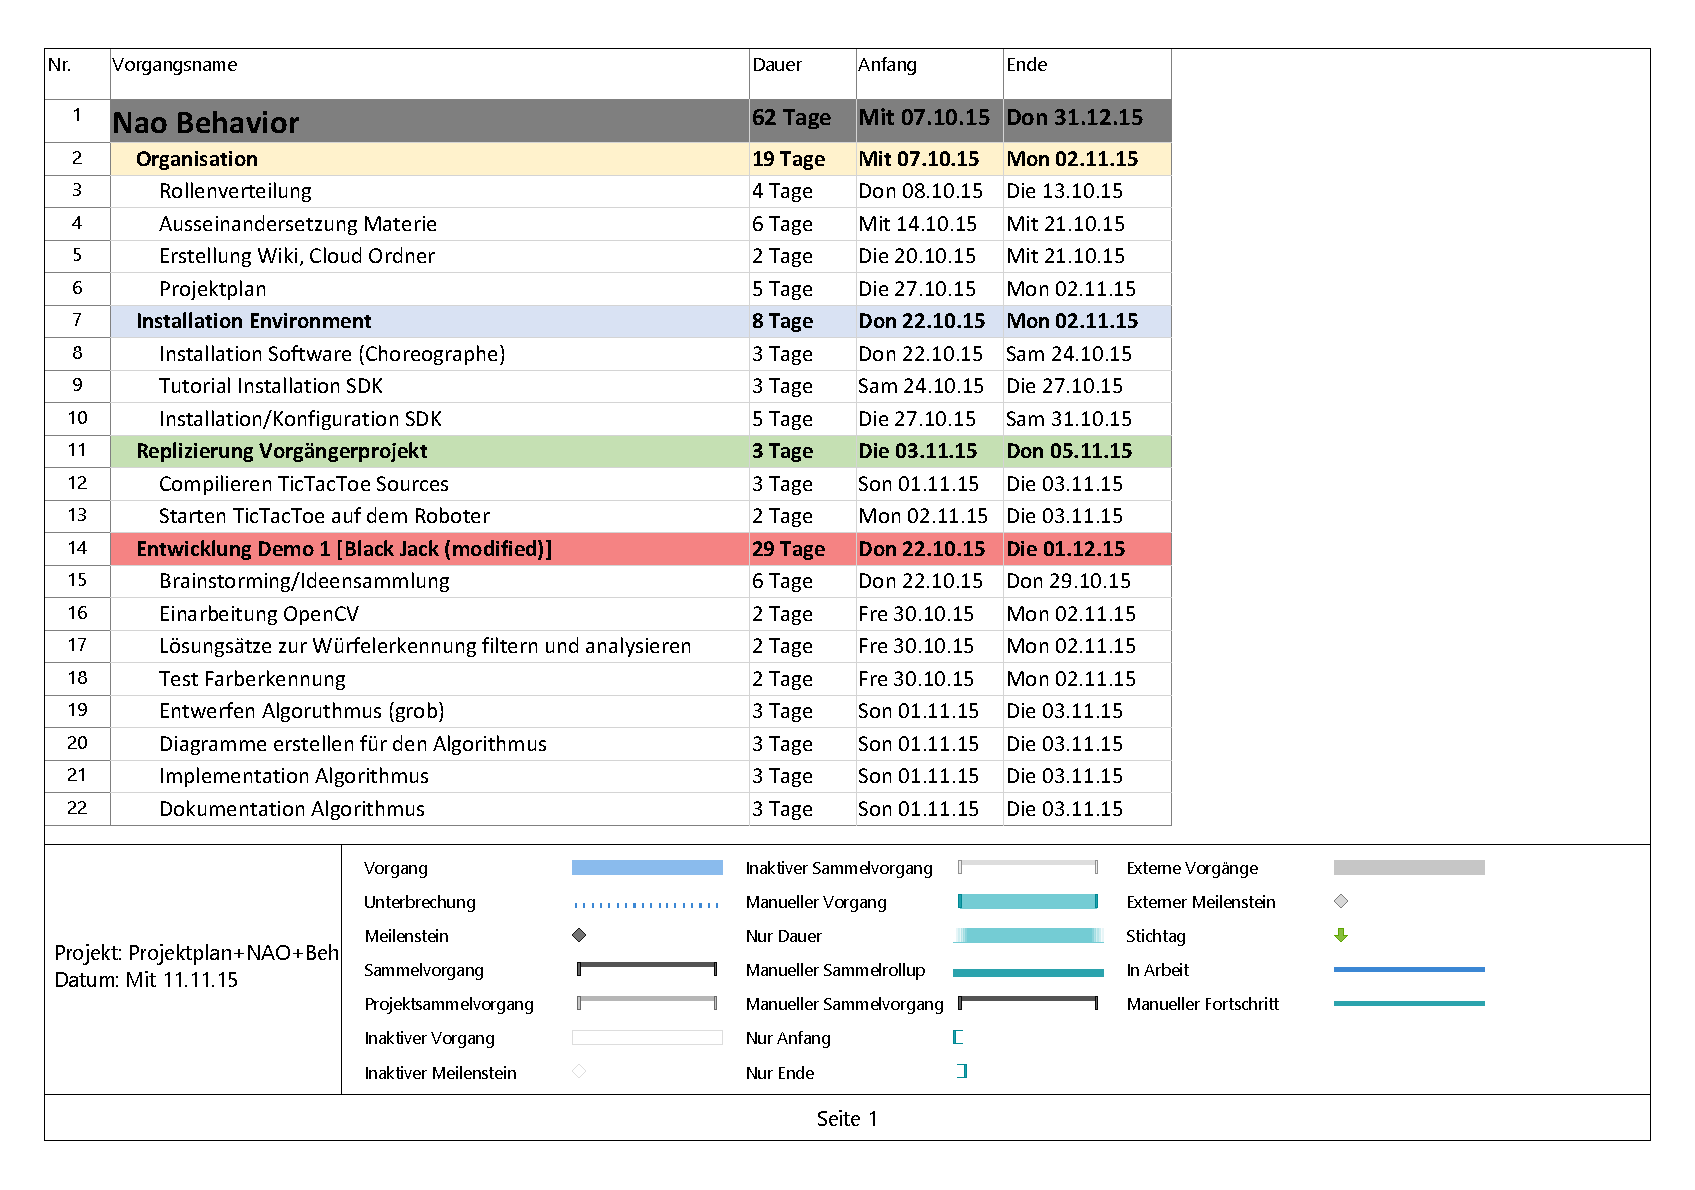
\includepdf[landscape=true,pages=-]{src/pictures/projektplan.pdf}
        \label{apx:projektplan}


\end{appendix}
